%----------------------------------------------------------------------------------------
%	PACKAGES AND THEMES
%----------------------------------------------------------------------------------------

\documentclass{beamer}
\usepackage{ragged2e}
\justifying

\mode<presentation> {
\usetheme{CambridgeUS}
\usecolortheme{dolphin}
\setbeamertemplate{navigation symbols}{}}

\usepackage[utf8]{inputenc}
\usepackage[T1]{fontenc}
\usepackage[british]{babel}
\usepackage{amsmath,amsthm,amssymb,amsfonts}
\usepackage{enumerate}
\newcommand{\bm}{\boldsymbol}
\newcommand{\ds}{\displaystyle}
\newcommand{\mA}{{\mathbb A}}
\newcommand{\mB}{{\mathbb B}}
\newcommand{\mC}{{\mathbb C}}
\newcommand{\mD}{{\mathbb D}}
\newcommand{\mE}{{\mathbb E}}
\newcommand{\mI}{{\mathbb I}}
\newcommand{\mN}{{\mathbb N}}
\newcommand{\mQ}{{\mathbb Q}}
\newcommand{\mP}{{\mathbb P}}
\newcommand{\mR}{{\mathbb R}}
\newcommand{\mS}{{\mathbb S}}
\newcommand{\mZ}{{\mathbb Z}}
\newcommand{\cA}{{\mathcal A}}
\newcommand{\cb}{{\mathcal B}}
\newcommand{\cC}{{\mathcal C}}
\newcommand{\cE}{{\mathcal E}}
\newcommand{\cF}{{\mathcal F}}
\newcommand{\cG}{{\mathcal G}}
\newcommand{\cH}{{\mathcal H}}
\newcommand{\cI}{{\mathcal I}}
\newcommand{\cJ}{{\mathcal J}}
\newcommand{\cL}{{\mathcal L}}
\newcommand{\cM}{{\mathcal M}}
\newcommand{\cO}{{\mathcal O}}
\newcommand{\cP}{{\mathcal P}}
\newcommand{\cT}{{\mathcal T}}
\newcommand{\cU}{{\mathcal U}}
\newcommand{\cV}{{\mathcal V}}
\newcommand{\cZ}{{\mathcal Z}}
\newcommand{\sM}{{\mathscr M}}
\newcommand*{\defeq}{\mathrel{\vcenter{\baselineskip0.5ex \lineskiplimit0pt
                     \hbox{\scriptsize.}\hbox{\scriptsize.}}}%
                     =}
\usepackage{mathrsfs}

\usepackage[version=3]{mhchem}

\newcommand{\quotes}[1]{``#1''}

%----------------------------------------------------------------------------------------
% GRAPHICS
%----------------------------------------------------------------------------------------

\usepackage{graphicx}
\usepackage{tikz}
\usepackage{epstopdf}
\usepackage{color}
\definecolor{mygreen}{rgb}{0,0.6,0}
\definecolor{myred}{RGB}{139,0,0}
\definecolor{myblue}{RGB}{0,0,205}
\definecolor{myorange}{RGB}{255,140,0}
\usepackage{booktabs} % Allows the use of \toprule, \midrule and \bottomrule in tables

%----------------------------------------------------------------------------------------
%	TITLE PAGE
%----------------------------------------------------------------------------------------

\title[Combustion of rocket propellant]{Equilibrium for combustion of rocket propellant}
\author[Team Rocket]{A. Delgado, F. Granell, M. Llin\`as and J. Puig}
\institute[MMT]{Mathematical Models of Technology}
\date{Wednesday, 4th Oct 2015}

\begin{document}

\begin{frame}
\titlepage
\end{frame}

\begin{frame}
\frametitle{Overview}
\tableofcontents
\end{frame}

%----------------------------------------------------------------------------------------
%	PRESENTATION SLIDES
%----------------------------------------------------------------------------------------

\section{Statement of the problem}

%------------------------------------------------

\begin{frame}
\frametitle{Motivation}
\begin{itemize}
\item Rocket propellant is a material used by a rocket that reacts chemically, ejecting a reaction mass with
very high speed to produce thrust, and thus provide spacecraft propulsion.
\item The type of propellant varies depending on the type of rocket.
\item We focus on rockets that are propelled by means of combustion reactions, which are exothermic and which happen at high temperatures.
\item Under these conditions, the components dissociate, which makes the parameters of the reaction dicult to find.
\item Our aim is to determine the parameters of the reaction at the same time as we provide a full open-source solver for combustion problems involving a gas mixture with dissociation.
\end{itemize}
\end{frame}

%------------------------------------------------

\section{Preliminary concepts}

%------------------------------------------------

\subsection{Review of Kinetic Molecular Theory}

%------------------------------------------------

\begin{frame}
\frametitle{Basics I}
\begin{block}{Conservation of Mass Law}
In any chemical reaction, the sum of the masses of the reagents is equal to the sum of the masses of the products.
\end{block}
\begin{block}{Ideal Gases Law}
Given the pressure $P$, volume $V$ and temperature $T$ of an ideal gas,
\begin{equation*}
PV=nRT, \ R=0,082 \text{ atm}\cdot\text{L}\cdot\text{mol}^{-1}\cdot\text{K}^{-1},
\end{equation*}
where $n$ is the number of moles contained in the gas.
\end{block}
\end{frame}

%------------------------------------------------

\begin{frame}
\frametitle{Basics II}
\begin{block}{Dalton's Law of Partial Pressures}
The total pressure of a mixture of gases equals the sum of the partial pressures. Mathematically, given a mixture of $n$ gases in a container,
\begin{equation*}
P = \sum_{i = 1}^n P_i, \qquad P_i = n_i\frac{RT}{V} = n_i\frac{P}{n} = \frac{n_i}{n}P = \chi_i P.
\end{equation*}
\end{block}
\begin{block}{Molar fraction}
The molar fraction $\chi_i$ of the gas $i$ is
\begin{equation*}
\chi_i = \frac{n_i}{n} = \frac{P_i}{P} = \frac{V_i}{V}.
\end{equation*}
\end{block}
\end{frame}

%------------------------------------------------

\subsection{Review of Thermodynamics}

%------------------------------------------------

\begin{frame}
\frametitle{First Law of Thermodynamics}
The total energy of an isolated system is constant. Mathematically, we write
\begin{equation*}
\Delta U = Q + W,
\end{equation*}
where $U$ is the internal energy, $Q$ is the heat involved in the process and
\begin{equation*}
W = -P_{\text{ext}}\Delta V = -\Delta nRT
\end{equation*}
is the work performed through compression or expansion of the system, where $P_{\text{ext}}$ is the pressure that the exterior exerts upon the gas and $\Delta n$ is the variation in the number of moles.
\end{frame}

%------------------------------------------------

\begin{frame}
\frametitle{Constant-volume and constant-pressure reactions}
\begin{block}{Enthalpy}
Let us define the \textit{enthalpy} $H$ as
\begin{equation*}
H = U + PV.
\end{equation*}
\end{block}
It is important to notice that enthalpy is a thermodynamic potential, so in order to measure the enthalpy of a system, we must refer to a defined reference point. Therefore what we measure is the change in enthalpy, $\Delta H$.
\end{frame}

%------------------------------------------------

\begin{frame}
\frametitle{Particular cases of enthalpies}
\begin{itemize}
\item Standard enthalpy of reaction $\Delta H_r^0$
\item Standard enthalpy of formation $\Delta H_f^0$ for 1 mol of a substance from the basic elements in the standard states of reference
\item Reticular energy
\item Bond dissociation energy
\end{itemize}
One may calculate
\begin{equation*}
\Delta H_r^0=\sum_{p\in P}v_p\Delta H_f^0(p) - \sum_{r\in R} v_r\Delta_f^0(r),
\end{equation*}
where $P$ and $R$ are the set of products and reagents, respectively, and $v_p$ and $v_r$ are the stoichiometric coefficients in the reaction.
\end{frame}

%------------------------------------------------

\begin{frame}
\frametitle{Enthalpy diagrams}
\begin{block}{Hess's Law}
If a reaction can be expressed as the sum of several elementary reactions, then the variation in the enthalpy of the reaction can be calculated adding up the variations in the enthalpy of each elementary reaction.
\end{block}
\begin{figure}
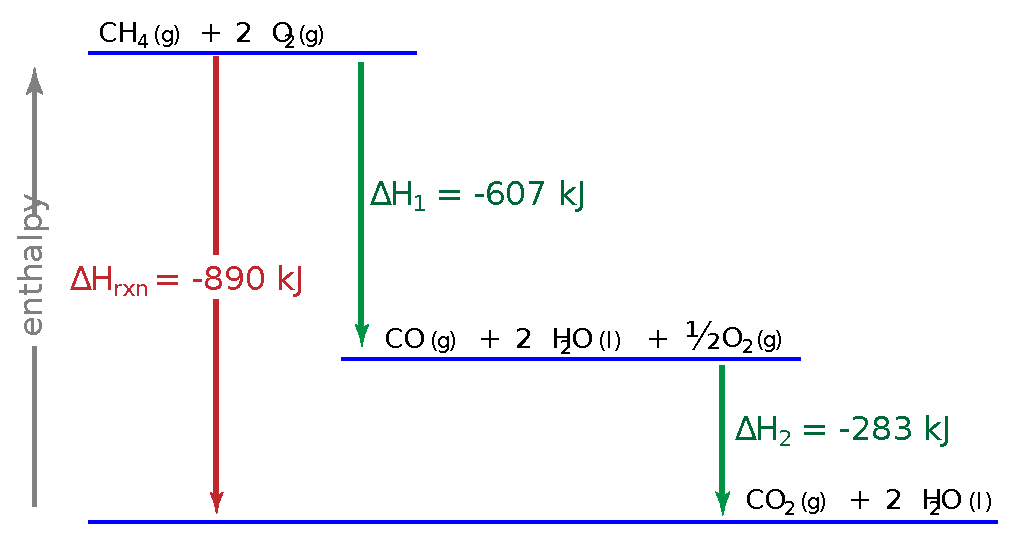
\includegraphics[width=0.8\linewidth]{hess-law}
\end{figure}
\end{frame}

%------------------------------------------------

\begin{frame}
\frametitle{Second and Third Laws of Thermodynamics}
\begin{block}{Second Law of Thermodynamics}
Given a thermodynamical system, the change in entropy can be expressed as
\begin{equation*}
\Delta S = \frac{Q_{\text{rev}}}{T},
\end{equation*}
where $Q_{\text{rev}}$ is the heat that intervenes in a reversible process. Alternatively,
\begin{equation*}
\Delta S_{\text{universe}} = \Delta S_{\text{system}} + \Delta S_{\text{environment}}>0.
\end{equation*}
\end{block}
\begin{block}{Third Law of Thermodynamics}
The entropy of a perfect pure crystal at 0 K is zero.
\end{block}
\end{frame}

%------------------------------------------------

\begin{frame}
\frametitle{Spontaneity} 
If we assume that the variation in the entropy of the environment is due to $-\Delta H_{\text{system}}$ and take into account the Second Law of Thermodynamics, we get $\Delta H_{\text{system}} - T\Delta S < 0$.
\begin{block}{Gibbs free energy}
We can then conveniently define
\begin{equation*}
G = H - TS.
\end{equation*}
\end{block}
\begin{block}{Criteria for predicting the nature of a thermodynamic process}
\begin{table}[h]
\begin{center}
\begin{tabular}{cccc}
   $\Delta H$ & $\Delta S$ & $\Delta G$ & Nature of the process  \\ \hline
   $-$ & $-$ & ? & spontaneous for small $T$\\
   $-$ & $+$ & $-$ & spontaneous\\
   $+$ & $+$ & ? & spontaneous for large $T$\\
   $+$ & $-$ & $+$ & non spontaneous\\
\end{tabular}
\end{center}
\end{table}
\end{block}
\end{frame}

%------------------------------------------------

\section{Our approach to the problem}

%------------------------------------------------

\begin{frame}
\frametitle{Sketch of the procedure}
\begin{itemize}
\item Chemical equilibrium is a state in which the species involved remain constant along time.
\item We aim to determine some properties about a chemical reaction given the reagents. In particular, we wish to determine whether the chemical equilibrium is attained in reactions of combustion.
\item There are infinitely many solutions and each one has an associated value for $G$.
\item We can formulate a minimisation convex problem for the Gibbs free energy.
\item The reaction that actually takes place is the one that has the minimum Gibbs free energy.
\end{itemize}
\end{frame}

%------------------------------------------------

\begin{frame}
\frametitle{What has been done so far}
\begin{itemize}
\item Creation of a whole package in a Matlab� environment. This one includes:
\begin{itemize}
\item the \texttt{HGS} function that calculates properties of mixtures of gases
\item the \texttt{fminineq} function that minimises the Gibbs free energy of a mixture of gases
\end{itemize}
\item In comparison to the Matlab's \texttt{fmincon} function, \texttt{fminineq} performs successfully in a variety of cases. However, it does not even provide similar results in others.
\end{itemize}
\end{frame}

%------------------------------------------------

\begin{frame}
\frametitle{What we intend to do}
\begin{itemize}
\item State an optimization problem for the Gibbs? energy.
\item Come up with a open-source (Python-based) numeric solving procedure for the problem.
\item Compare it to the existing MATLAB (HGS Chemical Equation Solver) solution.
\item Propose and explore improvements (speed, complexity, easy to use)
\item Document the solution and upload it into a public repository.
\end{itemize}
\end{frame}

%------------------------------------------------

%------------------------------------------------

\begin{frame}
\frametitle{What we have done so far}
\begin{itemize}
\item State an optimization problem for the Gibbs? energy.
\item Get familiar with the existing Matlab software (Burcat chemical elements database as well as the functions \texttt{fmincon}, \texttt{fminineq} and \texttt{hgs}).
\item Start to programme a python-based solver.
\end{itemize}
\end{frame}

%------------------------------------------------
\section*{}

%------------------------------------------------

\begin{frame}
\Huge{\centerline{Thanks for your attention!!}}
\begin{figure}

\includegraphics[width=0.5\linewidth]{team-rocket}
\end{figure}
\end{frame}

%----------------------------------------------------------------------------------------

\end{document}